\documentclass[10pt,a4paper]{article}

\usepackage[utf8]{inputenc}
\usepackage[T1]{fontenc}
\usepackage[francais]{babel}
\usepackage{url}
\usepackage{color}
\usepackage{verbatim}
\usepackage{amsmath,amssymb,amsfonts}
\usepackage{graphicx}
\usepackage[french]{algorithm2e}
\usepackage{geometry}
\geometry{hmargin=2.5cm, vmargin=2.5cm}

\title{TP CSE : Allocation mémoire}
\author{Line \bsc{POUVARET}, Mickaël \bsc{TURNEL}}
\date{2015-2016}



\begin{document}
\maketitle

\section{Choix justifiés d'implantation}
\begin{figure}[!ht]
	\center
	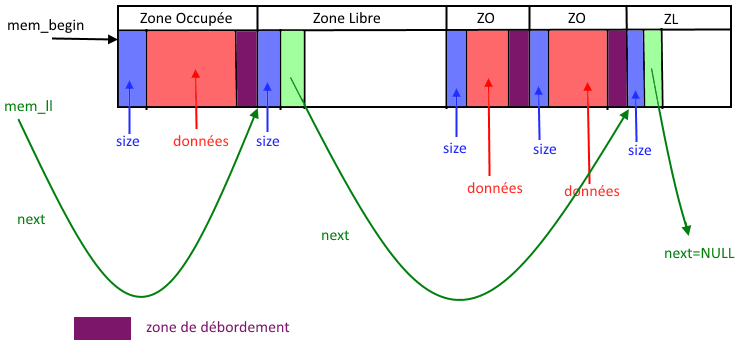
\includegraphics[width=15cm]{memoire.png}
 	\caption{Schéma représentant le fonctionnement de notre allocateur mémoire}
\end{figure}

La taille au début de chaque zone correspond bien à la taille de toute la zone en question donc : size + données + débordement pour une zone occupée et size + next + la zone vide pour une zone libre. Ceci permet un parcours plus simple de la mémoire.\\
Nous avons implémenté un padding (cf. Fonctionnalités) afin d'éviter d'avoir des zones libres inutilisables.
\section{Fonctionnalités}
\begin{itemize}
	\item Nous avons implémenté les trois stratégies First Fit, Best Fit, Worst Fit.
	\item Nous avons choisi d'implanter le padding lors de l'allocation d'une zone mémoire. Lorsque la taille de la zone libre - la taille demandée alignée + la taille de \textbf{size\_t} + la taille de la zone de débordement est inférieure à la taille d'une structure de zone libre alors on prend toute la zone libre. Ce qui nous évite des zones libres trop petites et inutilisables.
\end{itemize}

\section{Limites de notre code}
	Pour notre implémentation de Best Fit, on effectue un parcours de toute la liste alors qu'il existe des façons plus efficaces (mais plus compliquées) de déterminer la taille minimum à allouer dans la liste des zones libres.
	
\section{Extensions}

\subsubsection*{Ce que nous avons implanté}
\begin{itemize}
	\item Nous avons mis en place une zone de débordement à la fin de chaque zone occupée d'une taille d'un \textbf{long} contenant la valeur 0xDEADBEEF que l'on ajoute à la taille demandée par l'utilisateur avant d'aligner celle-ci. Lors d'un mem\_free, si cette valeur n'est plus à la fin de cette zone, alors on a eu un débordement et on exécute \textbf{abort}.
	\item Nous avons implémenté la gestion du multi-threading : nous avons un mutex qui s'appelle \textbf{lock} que nous verrouillons lors d'un mem\_alloc ou d'un mem\_free qui empêche que ces deux fonctions soient exécutées simultanément.
\end{itemize}
\subsubsection*{Ce que nous aurions voulu implanter}
\begin{itemize}
	\item Nous aurions bien voulu implanter la stratégie du Next Fit (qui correspond à un First Fit avec une liste circulaire).
	\item Nous aurions également bien voulu réaliser la compatibilité avec valgrind.
\end{itemize}

\section{Tests realisés}
En plus du programme memtest fourni, nous avons réalisé trois jeux de test.
Ces trois programmes de test sont lancés avec memtest en effectuant la commande \textbf{make tests}

\begin{itemize}
	\item \textbf{test\_fit} : prend comme argument 1, 2 ou 3. 1 = First Fit, 2 = Best Fit, 3 = Worst Fit. Le programme fera une série d'allocations de libérations pour mettre la mémoire dans un état spécifique pour ensuite effectuer une allocation qui fait que l'état de la mémoire sera différent selon la stratégie choisi. Ceci est utile pour montrer le fonctionnement de chaque stratégie.
	\item \textbf{test\_debordement} : ne prend pas d'argument. Ce programme réalise une allocation mémoire classique, on va allouer un tableau de la taille de l'alphabet classique et chaque case du tableau contiendra une lettre de l'alphabet. Puis, on effectue une autre allocation de 100 entiers et on en affecte 101 dans la zone allouée ce qui conduit à un abort au moment de l'appel de mem\_free car celle-ci détectera un débordement.
	\item \textbf{test\_thread} : ne prend pas d'argument. On crée un thread dans lequel on va effectuer 25 allocations aléatoires puis libérer celles-ci. En même temps, le processus principal va lui aussi lancer 35 allocations aléatoires et libérer celles-ci puis attendre la fin du thread pour enfin afficher l'état de la mémoire (qui normalement devrait être une seule zone libre si tout s'est bien passé). Une succession aléatoire d'allocations et de libérations dans ce test aurait permis de rendre le test plus efficace.
\end{itemize}

\end{document}